% -*- mode: fundamental -*-

% Slides accompanying "Learn RISC-V CPU Implementation and BSV" book
% Copyright (c) 2024 Rishiyur S. Nikhil, All Rights Reserved

% -*- mode: fundamental -*-

% Slides accompanying "Learn RISC-V CPU Implementation and BSV" book
% Copyright (c) 2024 Rishiyur S. Nikhil, All Rights Reserved

% This is a preamble shared by all the slide decks

\documentclass[10pt, aspectratio=169]{beamer}

% \documentclass[17pt]{beamer}

% Avail. font sizes: 8pt, 9pt, 10pt, 11pt, 12pt, 14pt, 17pt, 20pt.
% Default font size is 11pt (= 22pt in full screen mode).

\usepackage{verbatim}
\usepackage{fancyvrb}
\usepackage{listings}

% ================================================================
% Themes

\usetheme{Madrid}          % Line at bottom: Author (affiliation), OptTitle, Conf, page 

% \usetheme{Copenhagen}    % Same as Madrid except bottom line: Author, OptTitle

% \usetheme{Berkeley}    % Takes up 1-inch border on left and top

% ----------------
% colorthemes
% (default), beaver, beetle, seahorse, wolverine

\usecolortheme{seahorse}

% ================================================================
% Customization: show table of contents before each section
% Use \AtBeginSubsection    to show before each subsection

% \AtBeginSection[]
% {
%   \begin{frame}
%     \frametitle{Table of Contents}
%     \tableofcontents[currentsection]
%   \end{frame}
% }

% ================================================================

% ----------------
% The bsc compiler and BSV language
\newcommand{\bsc}{\emph{bsc}}
\newcommand{\BSV}{\bf{BSV}}
% ----------------
% ITALICISE WORDS
\newcommand{\ie}{\emph{i.e.,}}
\newcommand{\eg}{\emph{e.g.,}}
\newcommand{\Eg}{\emph{E.g.,}}
\newcommand{\etc}{\emph{etc.}}
\newcommand{\via}{\emph{via}}
\newcommand{\vs}{\emph{vs.}}

% ----------------
% EMPTY BOXES OF VARIOUS WIDTHS, FOR INDENTATION

\newcommand{\hm}{\hspace*{1em}}
\newcommand{\hmm}{\hspace*{2em}}
\newcommand{\hmmm}{\hspace*{3em}}
\newcommand{\hmmmm}{\hspace*{4em}}

% ----------------
% Convenient widths

\newlength{\hlessmm}
\setlength{\hlessmm}{\textwidth}
\addtolength{\hlessmm}{-2em}

\newlength{\hlessmmm}
\setlength{\hlessmmm}{\textwidth}
\addtolength{\hlessmmm}{-3em}

\newlength{\hlessmmmm}
\setlength{\hlessmmmm}{\textwidth}
\addtolength{\hlessmmmm}{-4em}

% ================================================================
% Title page

\title[Learn CPU design \& BSV]{Learn RISC-V CPU Implementation and BSV}

\subtitle{(BSV: a High-Level Hardware Design Language)}

\author[{\copyright} R.S.Nikhil]{Rishiyur S.~Nikhil}
% \institute{Bluespec, Inc.}

% Date is set differently in each slide deck

% \logo{
\includegraphics[height=0.6cm]{../Figures/Bluespec_Logo_2022-10}}

% End of preamble
% ****************************************************************


\date{L5: {\BSV} Structs; Memory requests and responses}

% ****************************************************************

\begin{document}

% ================================================================

\begin{frame}
 \titlepage

 \begin{center}
  
\includegraphics[height=1cm]{Bluespec_Logo_2022-10}
 \end{center}

\end{frame}

% ================================================================

% -*- mode: fundamental -*-

% ================================================================

\begin{frame}[fragile]
\frametitle{Reminders}

\footnotesize

Please git clone: \url{https://github.com/rsnikhil/Learn_Bluespec_and_RISCV_Design} \\
(git pull for latest version).  Repsitory structure:

\vspace{1ex}

\begin{minipage}{0.5\textwidth}\scriptsize
\begin{Verbatim}[frame=single, numbers=left]
    ./Book_BLang_RISCV.pdf
      Slides/
          Slides_01_Intro.pdf
          Slides_02_ISA.pdf
          ...
      Exercises/
          Ex-03-A-Hello-World/
          Ex-03-B-Top-and-DUT/
          ...
      Code/
          src_Top/
          src_Drum/
          src_Fife/
          src_Common/
          ...
      Doc/Installing_bsc_Verilator_etc.{adoc,html}
\end{Verbatim}
\end{minipage}
\hm
\begin{minipage}{0.45\textwidth}
\begin{itemize}

 \item Slides and Exercise are numbered in sync with book Chapter numbers.

 \item For Exercises, please see Appendix E of the book.  Some (not
       all) exercises have associated code in the {\tt Exercises/}
       directory.

\end{itemize}
\end{minipage}

\vspace{2ex}

To compile and run the code for exercises, Drum and Fife, please make sure you have installed:

\begin{itemize}

 \item \emph{bsc} compiler (see \url{https://github.com/B-Lang-org/bsc})

 \item Verilator compiler (see \url{https://www.verilator.org/})
\end{itemize}

\footnotesize

\end{frame}

% ================================================================

\begin{frame}
\frametitle{Chapter Roadmap}

\footnotesize

\begin{center}
\frame{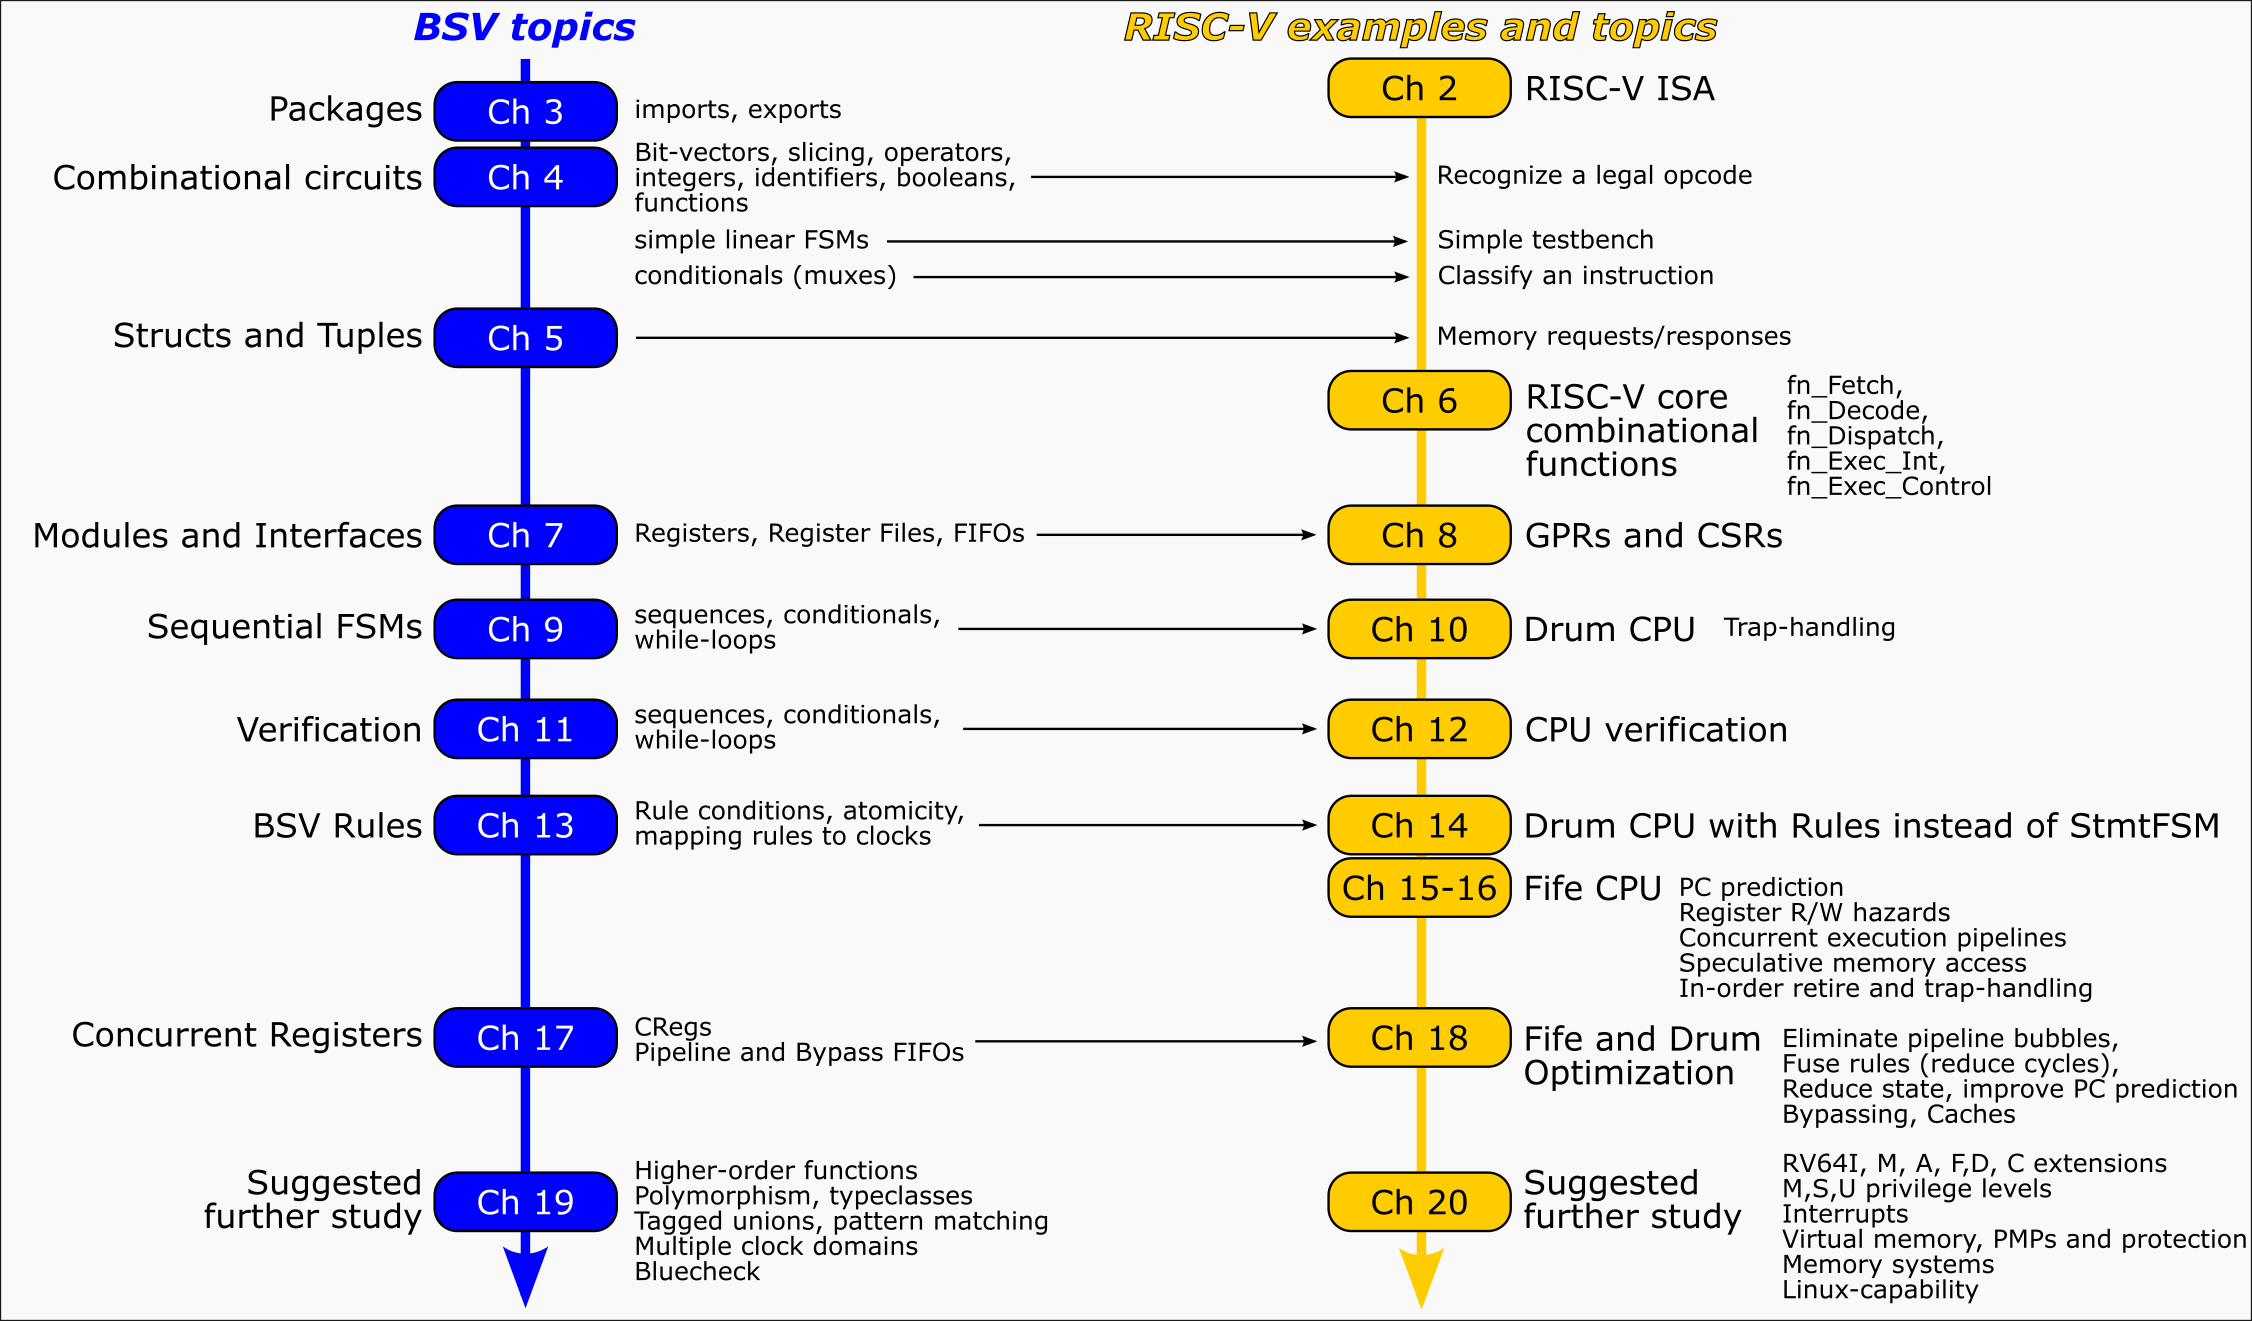
\includegraphics[height=0.825\textheight]{Fig_Chapter_Roadmap}}
\end{center}

\end{frame}

% ================================================================


% ================================================================

\begin{frame}
\frametitle{Flow of information between stages in Drum and Fife}

\footnotesize

\begin{center}
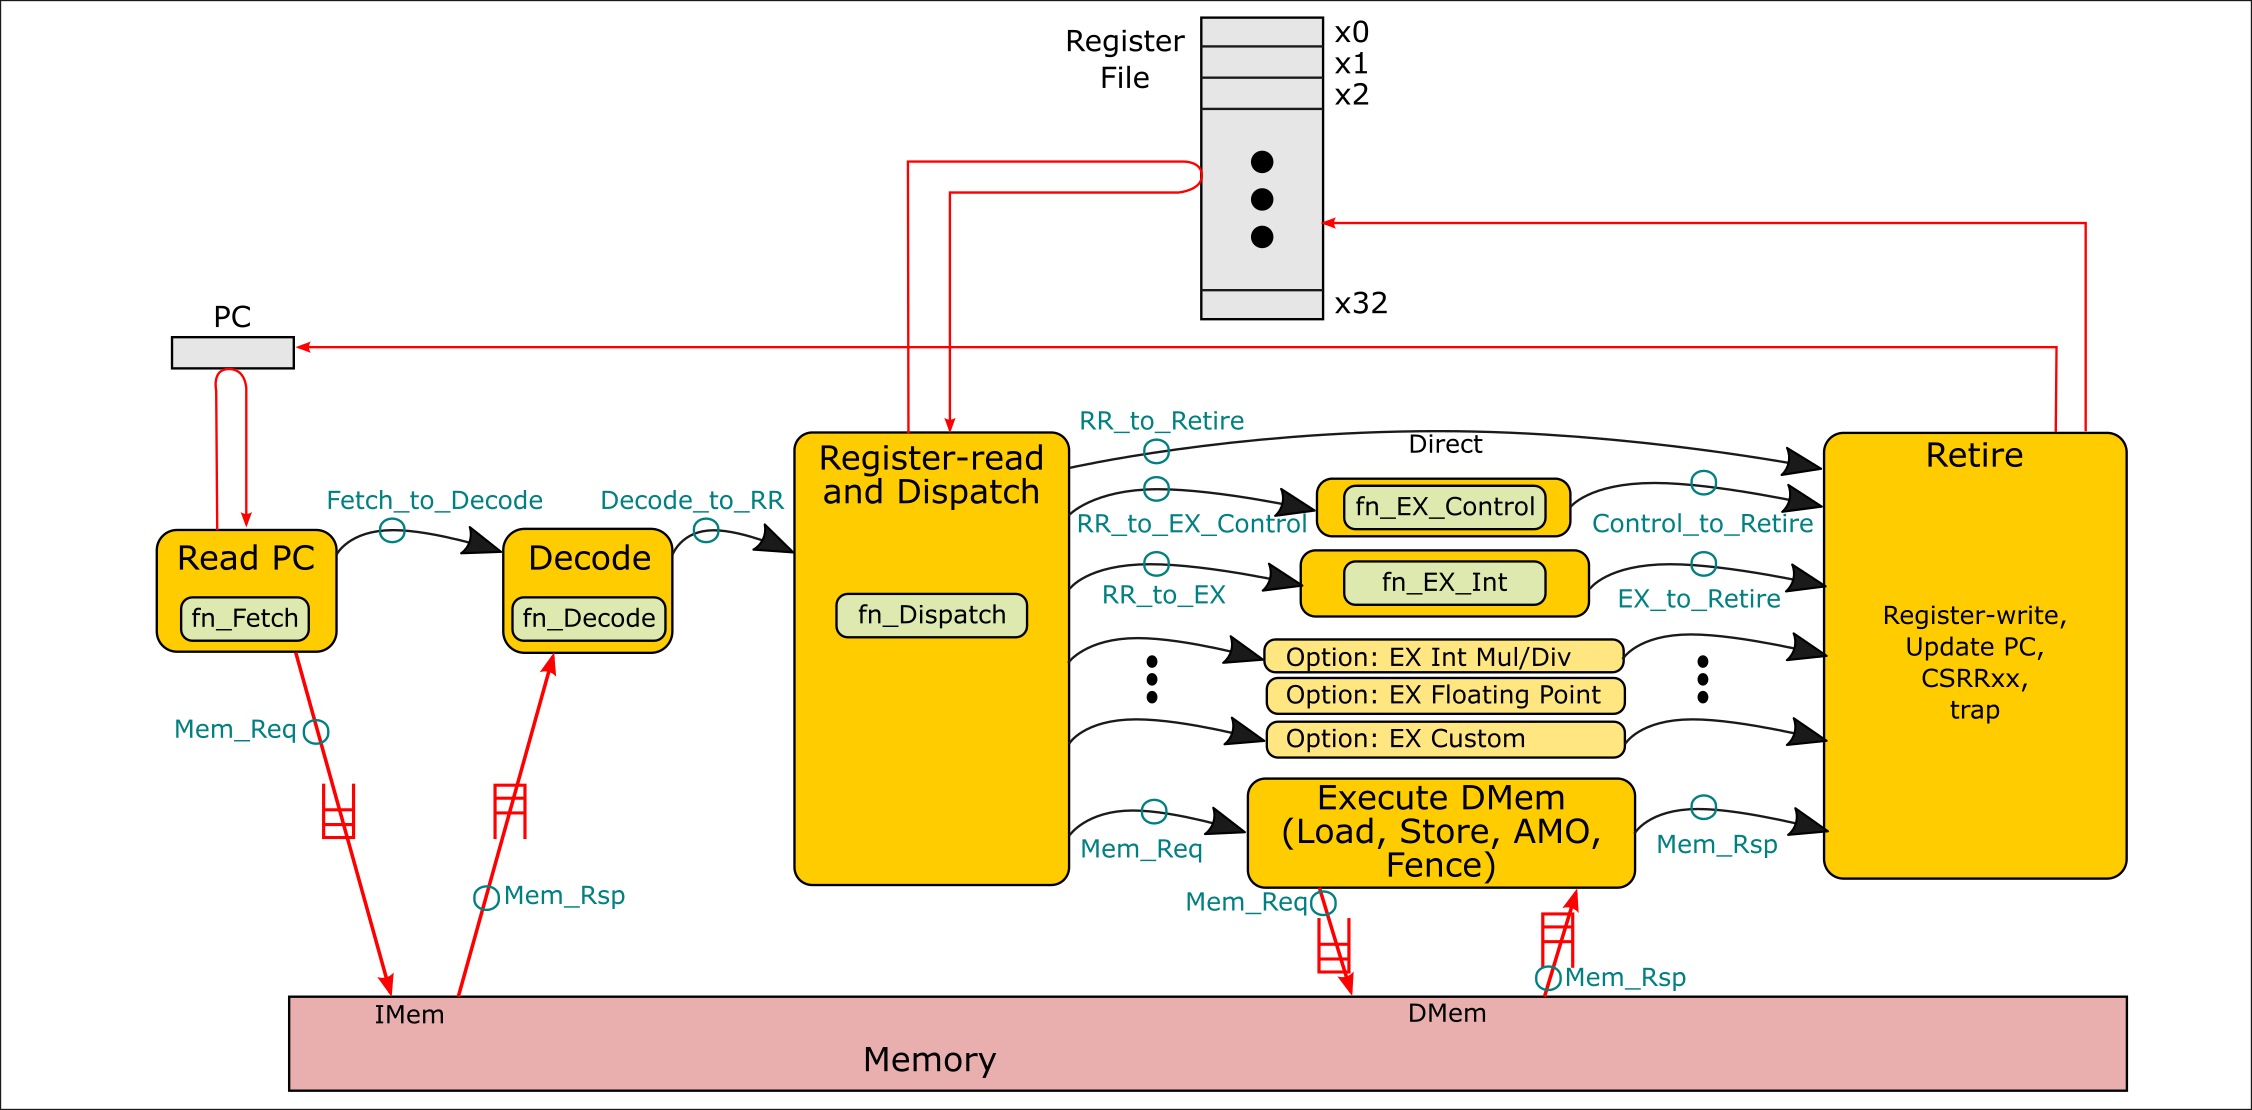
\includegraphics[height=0.6\textheight]{Fig_Instr_Exec_w_structs}
\end{center}

\vspace*{2ex}

The green annotations indicate the type of information flowing on each arrow.

Each of these is a ``{\tt struct}'' type (also known as a ``record''):
a grouping of \emph{fields} of heterogeneous types.

\end{frame}

% ================================================================

\begin{frame}[fragile]
\frametitle{Memory requests}

\footnotesize

\SHOWCODE{../Code_Extracts/Mem_Req.tex}

\vspace{2ex}

We will discuss {\tt Mem\_Req\_Type} and {\tt Mem\_Req\_Size} in some
following slides (they are just small bit-width scalars).

We will discuss the choice of 64 bits for {\tt addr} and {\tt data} in
some following slides.

\vspace{1ex}

The {\tt data} field is only relevant when communicating data from the
CPU to memory (STORE and AMO instructions).

\vspace{2ex}

When communicating 1, 2 and 4 bytes, these are in the
least-significant bytes of the {\tt data} field.

\PAUSE{\vspace{4ex}}

Note, we do not say ``{\tt deriving (Eq)}'' because we have no
occasion to compare two entire Memory Requests for
equality/inequality.

\end{frame}

% ================================================================

\begin{frame}[fragile]
\frametitle{{\BSV}: struct expressions to construct struct values}

\footnotesize

\begin{Verbatim}[frame=single, numbers=left]
   Mem_Req x = Mem_Req {req_type: funct5_LOAD,
                        size:     MEM_SIZE_4B,
                        addr:     'h_8000_0000,
                        data:     ?,
                        ...   };
\end{Verbatim}
The right-hand side is a ``struct expression'' whose value is a struct value.

\vspace{1ex}

If a field is left undefined, {\bsc} will warn while compiling.

\PAUSE{\vspace*{4ex}}

Some shorthands: ``{\tt let}'' and don't-care values:

\vspace*{2ex}

\begin{Verbatim}[frame=single, numbers=left]
   let  x   =  Mem_Req {req_type: funct5_LOAD,
                        size:     MEM_SIZE_4B,
                        addr:     'h_8000_0000,
                        data:     ?,
                        ...   };
\end{Verbatim}

\end{frame}

% ================================================================

\begin{frame}[fragile]
\frametitle{{\BSV}: Accessing and updating struct fields}

\footnotesize

These notations are standard in many programming languages.

\vspace{5ex}

Accessing fields:
\begin{Verbatim}[frame=single, numbers=left]
   x.req_type
   x.size
\end{Verbatim}

\vspace{5ex}

Updating fields:
\begin{Verbatim}[frame=single, numbers=left]
   x.req_type = MEM_REQ_STORE;
   x.data     = ... new value ... ;
\end{Verbatim}

\end{frame}

% ================================================================

\begin{frame}[fragile]
\frametitle{{\BSV}: Bit-representation of struct values}

\footnotesize

\begin{itemize}

 \item Because we said ``{\tt deriving (Bits)}'', {\bsc} will
       automatically pick a hardware representation of this struct as
       a bit-vector, by simply concatenating the bit-representations
       of the fields.  So, the size of the bit-vector for a struct
       value is the sum of the sizes of the bit-vectors for the
       fields.

 \PAUSE{\vspace{4ex}}

 \item If we wanted a different, custom representation, we omit ``{\tt
       deriving (Bits)}'', and there is a way (``Typeclass
       Instances'') to specify exactly what we want.

\end{itemize}

\end{frame}

% ================================================================

\begin{frame}[fragile]
\frametitle{{\BSV}: printing/logging struct values (for debugging)}

\footnotesize

We can print a struct value directly, {\eg}

\begin{Verbatim}[frame=single, numbers=left]
    Mem_Req mem_req;
    ...
    $display ("mem_req is: ", mem_req);
\end{Verbatim}

\vspace{5ex}

This will just print the hexadecimal notation for the full bit-vector
representing the struct.  This can be difficult to read:

\begin{itemize}
 \item Some structs are large (hundreds of bits!)

 \item Field boundaries may not align with hexadecimal bit boundaries
       (every 4 bits), and so correlating the hex digits to the fields
       can be tedious.
\end{itemize}

\end{frame}

% ================================================================

\begin{frame}[fragile]
\frametitle{{\BSV}: printing/logging struct values (for debugging)}

\footnotesize

Because we said ``{\tt deriving (FShow)}'', {\bsc} will automatically
define an ``{\tt fshow()} function for this struct, that will print
each field separately.

\vspace{2ex}

\begin{Verbatim}[frame=single, numbers=left]
    Mem_Req mem_req;
    ...
    $display ("mem_req is: ", fshow (mem_req));
\end{Verbatim}

\PAUSE{\vspace{5ex}}

If we wanted way to print the struct in a custom format, we omit
``{\tt deriving (FShow)}'', and there is a way (``Typeclass
Instances'') to define {\tt fshow()} to print what we want.

\end{frame}

% ================================================================

\begin{frame}[fragile]
\frametitle{Memory requests: {\tt Mem\_Req\_Type}}

\footnotesize

We could define the memory request-type as an {\tt enum}:
\begin{Verbatim}[frame=single, numbers=left]
typedef enum { MEM_REQ_LOAD, MEM_REQ_STORE} Mem_Req_Type
deriving (Bits, FShow, Eq);
\end{Verbatim}

However, looking ahead to future support of the ``A'' extension
(Atomic Memory Ops (AMOs), see Unprivileged ISA Spec p.132), we
observe that the ISA defines a 5-bit code in the instruction for each
AMO op.  If we use these 5 bits as-is, it will simplify decoding.  So,
we use 5 bits for the memory request-type:

\vspace{2ex}

\SHOWCODE{../Code_Extracts/Mem_Req_Type.tex}

\vspace{4ex}
and we pick two 5-bit codes that are unused by the AMO ops for LOAD and STORE:

\vspace{2ex}

\SHOWCODE{../Code_Extracts/funct5_MEMOPs.tex}

\end{frame}

% ================================================================

\begin{frame}[fragile]
\frametitle{Memory requests: {\tt Mem\_Req\_Size}}

\footnotesize

\SHOWCODE{../Code_Extracts/Mem_Req_Size.tex}

\PAUSE{\vspace{2ex}}

Why {\tt MEM\_8B}?  (RV32I can only LOAD/STORE bytes (1 byte),
halfwords (2 bytes) and words (4 bytes).)

\PAUSE{\vspace{1ex}}

This is with an eye towards future extension of our implementation:

\begin{itemize}

 \item If we support the D ISA extension (double-precision floating
       point), we'll need to be able to load/store doublewords (8 bytes).
       This could be in RV32 or RV64.

 \item If we support RV64I, we'll need to be able to load/store
       doublewords (8 bytes).

 \PAUSE{\vspace{2ex}}

 \item Even though RV32I and RV64I instructions are $\leq$ 32-bits
       wide, Fetch may choose to fetch more bits on each memory
       access, effectively ``pre-fetching'' subsequent instruction and
       reducing the number of memory accesses.

\end{itemize}

\PAUSE{\vspace{2ex}}

Why is the {\tt addr} field 64 bits instead of 32?  This is again with
an eye towards future extension of our implementation:

\begin{itemize}

 \item If we support RV64I, addresses will be 64 bits.

 \PAUSE{\vspace{1ex}}

 \item Even in RV32, physical memory/devices can allocated be at
       addresses larger than the $2^{32}$ address space.

\end{itemize}

\end{frame}

% ================================================================

\begin{frame}
\frametitle{\EmojiExercise \hmm Exercise break}

Please see Appendix E, Section Ex-05-A-Structs.

\end{frame}

% ================================================================

\begin{frame}[fragile]
\frametitle{Memory responses}

\footnotesize

Memory responses may report an exception (misaligned access,
non-existent memory, ...).

\vspace{2ex}

\SHOWCODE{../Code_Extracts/Mem_Rsp_Type.tex}

\vspace{4ex}

\SHOWCODE{../Code_Extracts/Mem_Rsp.tex}

\vspace{1ex}

The {\tt data} field is only relevant when communicating data from
memory to the CPU (LOAD and LR instructions).  When communicating 1, 2
and 4 bytes, these are in the least-significant bytes of the {\tt
data} field.

\end{frame}

% ================================================================

\begin{frame}
\frametitle{\EmojiExercise \hmm Exercise break}

Please see Appendix E, Section Ex-05-B-Mem-Req-Rsp.

\end{frame}

% ================================================================

\begin{frame}[fragile]
\frametitle{{\BSV}: Tuples: pre-defined immutable structs with special notation}

\footnotesize

Constructing a 2-tuple value: Example:
\begin{Verbatim}[frame=single, numbers=left, label=from src\_Common/CSRs.bsv]
   function ActionValue #(Tuple2 #(Bool, Bit #(XLEN)))
            fav_csr_read (Bit #(12) csr_addr);
      ...
	 return tuple2 (exception, y);
   endfunction
\end{Verbatim}

\PAUSE{\vspace{2ex}}

Accessing struct components using predefined functions {\tt tpl\_$j$}:
\begin{Verbatim}[frame=single, numbers=left]
   let xy <- fav_csr_read (...);
   let exc = tpl_1 (xy);    // exc has type: Bool
   let v   = tpl_2 (xy);    // v   has type: Bit #(XLEN)
\end{Verbatim}

\PAUSE{\vspace{2ex}}

Accessing struct components using pattern-matching:
\begin{Verbatim}[frame=single, numbers=left]
   match { .exc, .v } <- fav_csr_read (csr_addr);
\end{Verbatim}

\end{frame}

% ================================================================

\begin{frame}[fragile]
\frametitle{``Harvard'' Architecture: Separating Instruction and Data Memory}

\footnotesize

\begin{minipage}{0.35\textwidth}

 Since the very days of computers, most computers have separate channels to memory:

 \begin{itemize}

  \item ``IMem'': for Fetch to read from instruction memory

  \item ``DMem'': for LOAD/STORE instructions to read/write data memory

 \end{itemize}

 Typically, IMem and DMem can be accessed concurrently.

To facilitate this concurrency, programs typically do not modify their
 own instructions with LOAD/STORE instructions.

\end{minipage}
\hm
\begin{minipage}{0.6\textwidth}

 \begin{center}
  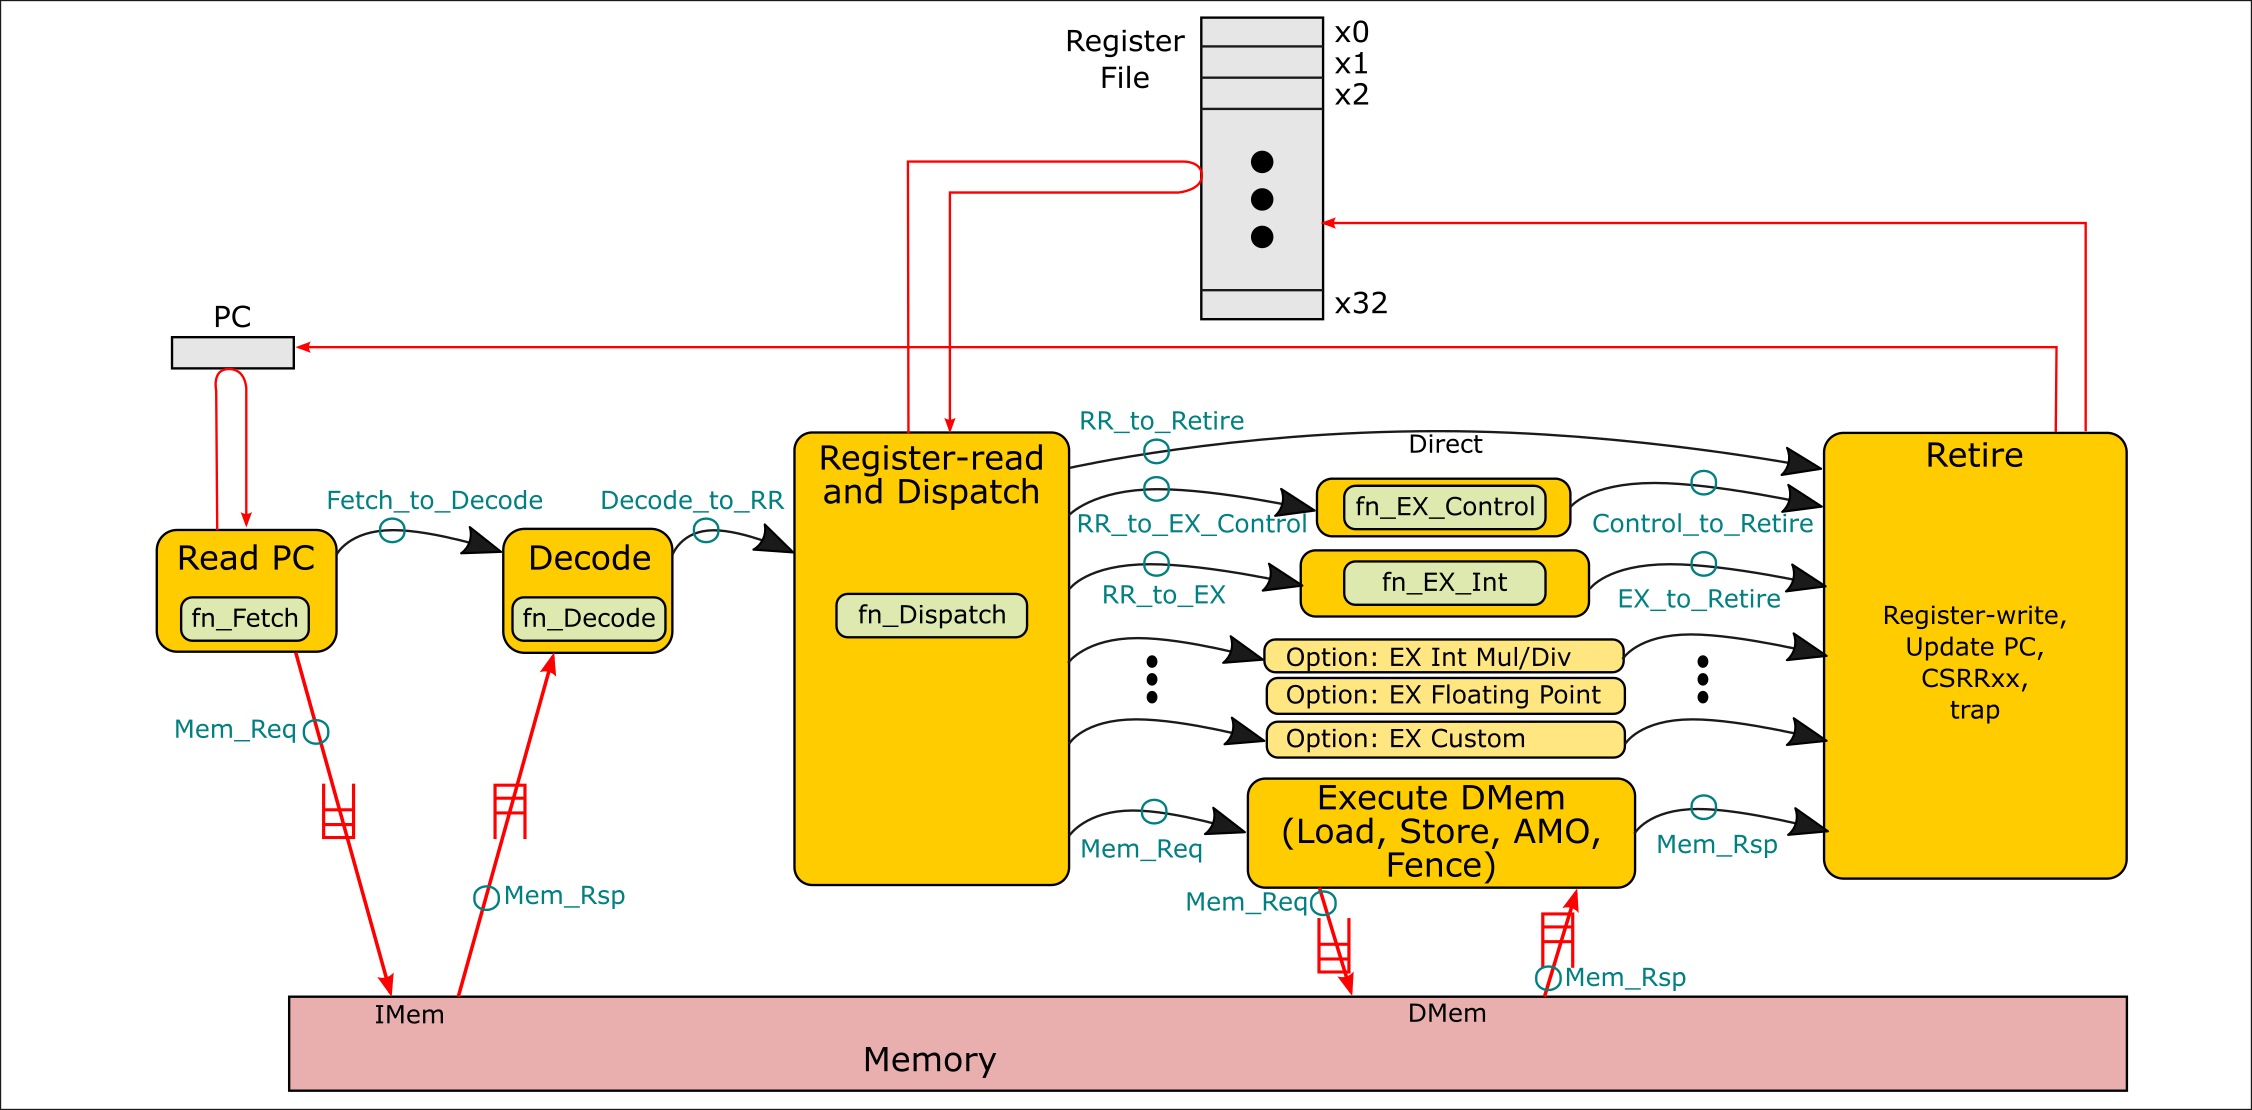
\includegraphics[width=\textwidth]{Fig_Instr_Exec_w_structs}
 \end{center}

\end{minipage}

\vfill

This organization is sometimes loosely called a ``Harvard Architecture''. \\
See: \hm \url{https://en.wikipedia.org/wiki/Harvard_architecture}.

\end{frame}

% ================================================================

% -*- mode: fundamental -*-

% Slides accompanying "Learn RISC-V CPU Implementation and BSV" book
% Copyright (c) 2024 Rishiyur S. Nikhil, All Rights Reserved

% This is a postamble shared by all the slide decks

% ================================================================

\begin{frame}

\begin{center}
  {\LARGE End}
\end{center}

\end{frame}

% ================================================================


% ****************************************************************

\end{document}
